\documentclass{UWNR_modeling}

%%%%%%%%%%%%%%%%%%%%%%%%%%%%%%%%%%%%%%%%%%%%%%%%%%%%%%%%%%%%%%%%%%%%%
\usepackage[T1]{fontenc}         % Use T1 encoding instead of OT1
\usepackage[utf8]{inputenc}      % Use UTF8 input encoding
\usepackage{microtype}           % Improve typography
\usepackage{booktabs}            % Publication quality tables
\usepackage{amsmath}
\usepackage{graphicx}
\usepackage{float}
\usepackage{tablefootnote}
\usepackage[exponent-product=\cdot]{siunitx}
\usepackage[colorlinks,breaklinks]{hyperref}
\usepackage{subcaption}
\hypersetup{linkcolor=black, citecolor=black, urlcolor=black}

\usepackage{lipsum}

\def\equationautorefname{Eq.}
\def\figureautorefname{Fig.}

%%%%%%%%%%%%%%%%%%%%%%%%%%%%%%%%%%%%%%%%%%%%%%%%%%%%%%%%%%%%%%%%%%%%%
% Insert authors' names and short version of title in lines below

\authorHead{YoungHui Park, Alexander Swenson}
\shortTitle{UWNR Model Improvements}

%%%%%%%%%%%%%%%%%%%%%%%%%%%%%%%%%%%%%%%%%%%%%%%%%%%%%%%%%%%%%%%%%%%%%
\begin{document}

\title{University of Wisconsin Nuclear Reactor Model Improvements}

\author{YoungHui Park\footnote{Graduate Research Assistant, Department of Engineering Physics}}
\author{Alexander Swenson\footnote{Undergraduate Research Assistant, Department of Engineering Physics}}
\author{Paul P.H. Wilson}
\affil{Computational Nuclear Engineering Research Group \\
  Department of Engineering Physics, University of Wisconsin-Madison\\
  1500 Engineering Drive, Madison, WI, 53706\\
  ypark234@wisc.edu; aaswenson@wisc.edu; paul.wilson@wisc.edu}
\maketitle

\begin{abstract}



\end{abstract}

%%%%%%%%%%%%%%%%%%%%%%%%%%%%%%%%%%%%%%%%%%%%%%%%%%%%%%%%%%%%%%%%%%%%%
\section{Introduction}
The University of Wisconsin Nuclear Reactor converted from HEU to LEU fuel in 2009. As part of the conversion process, an MCNP model was developed to predict flux distributions and depletion in the core. This core model included an unforeseen excess reactivity bias, resulting in an overestimate of core reactivity, and requiring the core configuration to be shuffled in 2011\cite{core_shuffle_report}. The original model was constructed by hand and in order to account for radial burnup in the fuel, and to include sufficient detail in the geometric featurse, the input file was over 17,000 lines long. Given the challenges in assessing the quality of such a long and complicated MCNP model, this project was designed build an MCNP model based on a minimal set of input quantities in a modular and repeatable fashion.  A Python code was developed to write the MCNP input file from fundamental reactor data, both geometric and material. The recent conversion to LEU fuel provides a unique opportunity to characterize fuel composition quite accurately in the core. The following is a description of that code and analysis of the resulting model.

The goals of this effort include:
\begin{itemize}
\item \textit{data provenance for quality assurance}: isolate the primary data describing geometry and materials to single locations and calculate all derived quantities in single locations,
\item \textit{modeling flexibility}: incorporate the ability to change the fuel element discretization as needed,
\item \textit{software flexibility}: support extension to alternative reactor physics analysis software,
\item maintainability: modularity and human readability of both the python scripts and the resulting MCNP input file, and
\item \textit{operational support}: facilitate various core configurations and fuel shuffling.
\end{itemize}

Section \ref{section:code_struct} describes many of the design decisions in both the Python script and the resulting MCNP input file.  Sections \ref{section:geometry} and \ref{section:materials} focus on specific details of the geometry and material descriptions, respectively.  Section \ref{section:analysis} then describes the results that arise from using this model, both in comparison to measured data and when subject to parametric analysis of some geometry and material quantities.

\section{Struggling for good section title}\label{section:structure}

The above stated goals lead to a number of important design decisions and features for both the reactor physics input file and the python scripts that generate such input files.  For the reactor physics input file, and specifically the MCNP input file targetted here, the geometric hierarchy suggests the use of specific software features that support such hiearchy, and a naming/numbering scheme that allows human readers to quickly determine aspects of that hierarchy.  For the python scripts, some modularity arises from the same geometric hiearchy, but additional modularity arises from best practices in software development, most importantly separation of concerns.  This section begins with a discussion of the features of the python script and input file that are largely separable from the geometric hiearchy, and then ends with a definition of that hierarchy including notes about how the individual features interact with that hierarchy.

\subsection{Python Code Structure}\label{ssection:code_struct}

The python scripts that ultimately generate the MCNP input files have been
constructed to support the goals indicated above.  In particular, modularity
across files has been used to ensure separation of concerns, thus isolating
different elements of the data and processing into logical units.  (see Figure
XXX)

\begin{itemize}
\item \texttt{reactor\_data.py}: fundamental quanitities that are rarely or never
  changing including dimensions, pin-to-bundle assignments and non-fuel
  material compositions
\item \texttt{core\_configuration.py}: a map showing how all 64 core positions are
  loaded with fuel bundles, reflector elements or water
\item three separate options for describing initial fuel compositions can be
  used interchangeably:
  \begin{enumerate}
  \item \texttt{as\_built\_slug\_averaged\_fuel\_comp.py}: fuel compositions are
    computed for each fuel slug (3 per pin) based on data provided by the fuel
    manufacturer
  \item \texttt{as\_built\_pin\_averaged\_fuel\_comp.py}: fuel compositions are
    averaged for each pin based on the above-calculated slug compositions
  \item \texttt{SAR\_fuel\_comp.py}: uniform composition defined by the Safety Analysis
    Report
  \end{enumerate}
\item \texttt{computed\_data.py}: quantities that are computed from the \texttt{reactor\_data},\\ \texttt{core\_configuration} and \texttt{*\_fuel\_comp} information such as derived dimensions, mapping of fuel slugs to core locations, etc.
\item \texttt{mcnp\_form.py}: specific syntax for generating cards for MCNP input files is isolated here and accessed from other locations through a common interface
\item \texttt{make\_uwnr.py}: the main script processes the input data and invokes software specific routines to generate output, taking advantage of the repeated structures present in the core model
\end{itemize}

\subsection{MCNP Input File Numbering Scheme}

Although the MCNP input file will be automatically generated by the scripts developed here, and will be too long ($\sim$12,000 lines) for a thorough manual review, various steps have been taken to facilitate the human readability of the file.   Most importantly, a numbering scheme was adopted to refer to cells, surfaces and materials so that their role in the model could be easily identified.  In addition, the Python scripts themselves are arranged in a hierarchical manner that is related to the hierarchical nature of a reactor core geometry.

The cell numbering scheme encodes a variety of information, including:
\begin{itemize}
\item where in the core hierarchy the cell exists,
\item the basic function of the cell within the core, and
\item the position in the core lattice (for fuel pins only).
\end{itemize}
\subsubsection{Cell and surface classification}

Regardless of the number of digits, the first digit indicates the role/function of the cell in the model.  This is generally true of surfaces as well, recognizing that some surfaces divide two cells with differing roles.  The following

\begin{tabular}{|c|l|}
\hline First Digit & Function\\\hline
1 & Pin active region, fuel\\
2 & Pin active region, nonfuel\\
3 & Reflector or water\\
4 & Control elements\\
5 & Structural components\\
6 & Thermal column\\
7 & Beam ports\\\hline
\end{tabular}

\subsubsection{Numbering convention for fuel pins: geometry and materials}

The seven digits in a fuel pin cell are used to indicate additional information according to the pattern, 
\texttt{[TRCPPMM]}, where

\begin{tabular}{|c|l|}
\hline
Position Code & Meaning \\\hline
T & Type     - 1 for fuel, 2 for nonfuel\\
R & Row      - Increasing number from East to West\\
C & Column   - Increasing number from North to South\\
P & Pin      - Number indicating pin location in a bundle\\
 & 01: South East\\
 & 02: South West\\
 & 03: North West\\
 & 04: North East\\
M & sub-pin region number (described in Section \ref{section:geometry})\\\hline
\end{tabular}

Similarly, the material identifiers for the fuel pins also encode additional information according to the pattern,
\texttt{[IIIIIMM]}, where 'I' represents the official 5-digit identification number of the fuel pin and 'M' indicates the same sub-pin region described in Section \ref{section:geometry}, below.

Importantly, the second through fifth (2-5) digits of a cell number refer to the position in the core while the first through fifth (1-5) digits of a material number refer to the official fuel pin identification number.  This facilitates shuffling of fuel as the material number is tied to the physical fuel element while the cell number is tied only to the position in the core.

\subsection{Repeated Structure Strategy}

Since the UWNR core model, like most reactor cores, is composed of repeated structures, both the python script and the resultant MCNP input file take advantage of this repetition.  Under this strategy, a so-called "master pin" is defined once and all other fuel pins are derived from this master pin.  So that each pin can contain a different material definition, to allow them to burnup independently, the "\texttt{like... but....}" capability was used to reduce the number of independent surface and cell definitions.  Each copy of a fuel pin has a modified material assignment, material density, and universe.  Each fuel pin is assigned to a universe that is identical to 4-digit number identical to digits 2-5 of the cell number.  

The lattice capability of MCNP is used to make fuel bundles from sets of 4 pins, but each lattice position is explicitly filled with a different universe corresponding to the appropriate pin.  Another layer of lattices is used to load each bundle into specific core positions.  Because the control elements have a thickness that is different from a unit cell of this lattice, three separate lattices are necessary: north, center, and south.  Each lattice is defined from the same set of surfaces, however, with the north and south lattices offset to their appropriate locations.  Each lattice contains 9 grid positions in the east-west direction.  The center lattice contains 3 grid positions in the north-south direction, while the north and south latices each contain 2.  (See Figure YY (8?))

The mapping of specific fuel pins, identified by their official UWNR ID, to bundles and then further to core positions is accomplished through simplified user input.  In particular, there is a mapping of bundle ID to core position using notation that corresponds to identifiers used by UWNR operators to refer to individual fuel bundles and to core locations.  This mapping is in \texttt{core\_configuration.py}, reflecting the fact that this level of configuration is easily modified during UWNR operation. In addition, there is a mapping of fuel pin ID to bundle ID and relative position within the bundle, again using notation that corresponds to UWNR operational practice.  This mapping is in \texttt{reactor\_data.py}, reflecting the fact that this level of configuration is rarely, if ever, changed during normal operating practices.  These two mappings are both necessary to establish the correspondence between specific pin IDs and core locations.


\subsection{Geometric Hierarchy}\label{ssection:geom_hier}

The UWNR's geometry follows a natural hierarchy, in which the full facility model includes many individual components as well as the reactor core itself, the core is arranged on a regular grid of with control elements, and each grid position may contain a bundle of individual fuel pins.  Similarly, the python script (as well as feature of the MCNP input file indicated below) is arranged to take advantage of this hierarchy.  In addition, where individual geometric components are repeated throughout the model, the software's methods take advantage of that repitition, both internally and in how those components are expressed in the resultant input file.

Surfaces and cells are made for components in a level. Then they are combined as a geometry level. Eventually, the levels are combined to build the whole reactor model.  The number of digits in a cell number indicates the level in this hierarchy at which the cell is defined.  Overall geometry structures are divided into the following 4 levels.
\begin{enumerate}
\item Pin level: Structures that make fuel pin sized components [seven (7) digit cell numbers]
	\begin{itemize}
	\item Master pin: An arbitrary fuel pin that creates geometries for fuel pins.
	\item Copy pin: Fuel pins other than the master pin. They are modeled to have the same geometry as the master pin to ensure consistency.
	\end{itemize}
\item Bundle level: Structures that make fuel bundle sized components [five (5) digit cell numbers]
	\begin{itemize}
	\item Fuel bundles: Arranged set of 4 fuel pins. They are positioned in core grids.
	\item Bottom adapters: Bottom portions of bundle elements that are made of Aluminum.
	\item Reflector elements: Graphite reflector elements positioned in core grids.
	\end{itemize}
\item Core level: Structures that make components in the core, excluding pin and bundle level. (Transient rod is included in this level along with other control elements.) [three (3) digit cell numbers]
	\begin{itemize}
	\item Transient rod: A type of control elements made with B4C. The Transient Rod is pneumatically actuated for transient experiments (i.e., pulses). It is positioned near the center of the core.
	\item Control shrouds(North and South): Aluminum shroud to guide safety blades and regulating blade. North shroud positioned between core north and center region, south shroud positioned between core center and south region, each with two water-filled rooms, east and west.
	\item Safety blades(\#1 - \#3): A type of control elements made with boral. (function?) They are positioned in east and west room of north shroud, east room of south shroud.
	\item Regulating blade: A type of control elements made with stainless steel. (function?) It is positioned in west room of south shroud.
	\item Core lattices: Lattice structures for each core region. Basically they are composed of grids.
	\item Core regions: Sectioned region in the core of the reactor. They are sectioned by the two control shrouds as north, center and south.
	\end{itemize}
\item Reactor level: Structures that make components in the reactor, excluding core level [three (3) digit cell numbers]
	\begin{itemize}
	\item Reactor pool: Water-filled space between the core and concrete shield.
	\item Thermal column: A type of experimental facilities on southern side of the core.
	\item Beam ports(\#1 - \#4): A type of experimental facilities extended from the outside of the core through reactor pool and concrete shield to the outter wall of concrete shield.
	\item Concrete shield: Biological shield surrounding reactor pool, experimental facilities and the core.
\end{itemize}
\end{enumerate}

\section{Model Geometry}\label{section:geometry}
Figure \ref{fig:fuel_xy} and Figure \ref{fig:fuel_yz} represent the modeled geometry of a fuel pin with arbitrary radial division, $R$, and axial division, $A$. In the figures, black strings represent the name of each surface, red numbers for the surface number and blue arrows for dimensions.  The number of radial and axial divisions is limited by their product, $R \cdot A \leq 99$, to accommodate the numbering scheme.  Later, analysis will show that this should allow for satisfactory discretization for this system. The fuel regions are numbered such that the radial segment varies more rapidly than the axial segment, or $MM = R\cdot(N_A-1) + (N_R-1)$, for radial segment, $N_R = 0, 1, 2, ..., (R-1)$, and axial segment, $N_A = 0, 1, 2, ..., (A-1)$.

\begin{figure}[H]
  \centering
  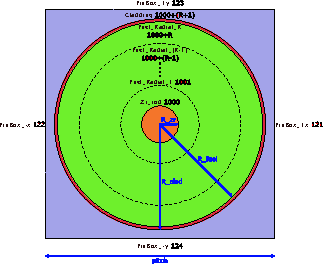
\includegraphics[width=4in]{fuel_xy.pdf}
  \caption{Fuel region, horizontal view.}
  \label{fig:fuel_xy}
\end{figure}

\begin{figure}[H]
  \centering
  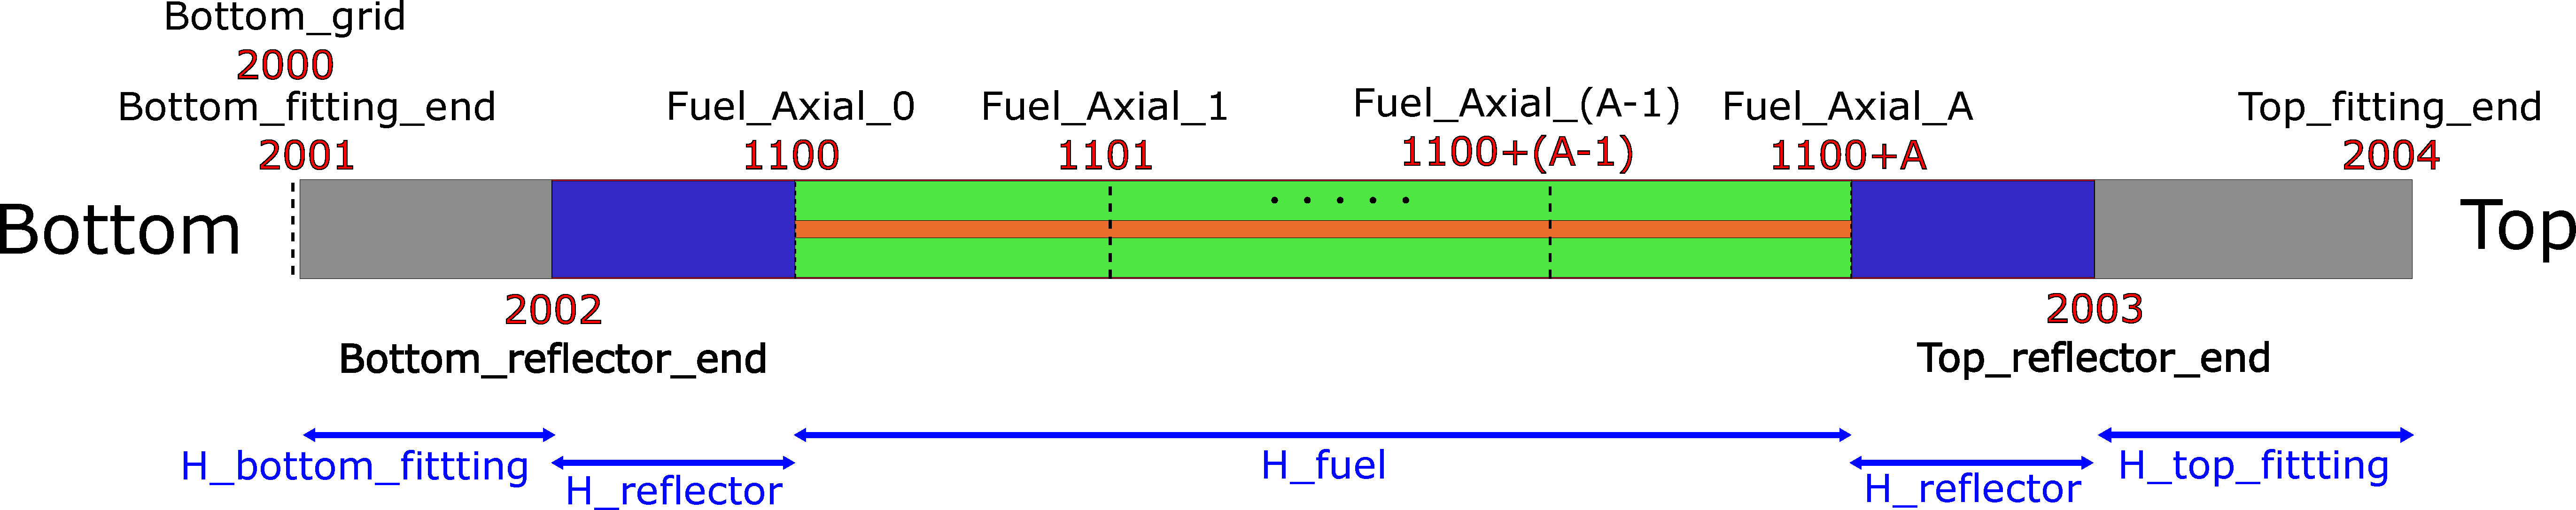
\includegraphics[width=7in]{fuel_yz.pdf}
  \caption{Fuel region, vertical view.}
  \label{fig:fuel_yz}
\end{figure}

On important modeling decision is that all fuel slugs are assumed to have the
same uniform length.  Data from the fuel vendor does indicate differing
lengths, but accommodating such differences was deemed to add unnecessary
complexity to the geometric model.  Instead, care has been taken to
appropriately combine the fixed slug length (and consequent volume) with the
vendor supplied masses for each slug to select an appropriate slug-specific
density, thus conserving total mass and total fissile mass.

Additional figures are provided in Appendix A.

\subsection{Control Element Height}

Control element height is adjusted through the use of 5 independent
transformations for which the z-translation is specified in the
\texttt{core\_configuration.py} file.  These translations are defined as being
relative to the fully inserted position, which is 1.5 inches below the bottom
of the active fuel for all control elements except the transient rod.  The
transient rod's fully inserted position is defined by reactor's licensing
basis, and subject to change.  The current fully inserted position is defined
in \texttt{reactor\_data.py}.

\section{Material Definitions}\label{section:materials}

At this time, three different estimations of the fuel initial compositions are available.  In each case, a mapping is generated between fuel pin ID and slug position to the material composition and density.  Different levels of approximation are invoked by importing different python files each with the same interface to provide this map.

\subsection{As-Built fuel composition}

The most exact representation of materials defines this fuel composition map based on slug-averaged data provideby the vendor\footnote{CERCA (subsidiary of AREVA)}. The following composition data are given for each of the three slug sections in a fuel pin.  This data is included as a version-controlled comma-separated values (CSV) file in the code repository.

\begin{tabular}{|c|c|l|}
\hline
Heading & Nomenclature & Description \\ \hline
Bundle & & Bundle number of corresponding pins\\
Pin & & Fuel ID number of a pin\\
Slug & & Slug section in a pin:'Top', 'Middle' or 'Bottom'\\
H/Zr atom ratio & $f_{a,H/Zr}$ & Atom ratio of hydrogen to zirconium atoms\\
Er wt\% & $100 \cdot f_{m,Er}$ & Mass fraction of elemental erbium [\%]\\
C wt\% & $100 \cdot f_{m,C}$ & Mass fraction of elemental carbon [\%]\\
Total mass & $m_{tot}$ & Total mass of a slug\\
Total U mass & $m_{U}$ & Total mass of uranium elements\\
U-235 mass & $m_{U235}$ & Mass of uranium-235 isotope\\ \hline
\end{tabular}

\textbf{Notation}
\begin{itemize}
\item $f_{a,X/Y}$ - atom ratio of component $X$ to $Y$ in a fuel slug,
\item $f_{m,X/Y}$ - mass ratio of component $X$ to $Y$ in a fuel slug,
\item $f_{m,X}$ - mass fraction of component $X$ (i.e. mass ratio of $X$ to total mass),
\item $m_X$ - mass of component $X$ in a fuel slug [g],
\item $M_X$ - Atomic mass of component $X$ [g/mol]
\end{itemize}

In addition to this data from the vendor, three quantites are taken from the
literature to represent impurities:
\begin{itemize}
\item $f_{m,U234/U235}$ : Industry accepted average value.
\item $f_{m,U236/U235}$ : Industry accepted average value.
\item $f_{m,Hf/Zr}$  : Texas A\&M University LEU Conversion Report \cite{xx}
\end{itemize}

Using the given data above, following material data are calculated.
\begin{eqnarray*}
m_{U234} &=& m_{U235} \cdot f_{m,U234/U235}\\
m_{U236} &=& m_{U235} \cdot f_{m,U236/U235}\\
m_{U238} &=& m_{U} - m_{U235} - m_{U234} - m_{U236}\\
m_{C} &=&  f_{m,C} \cdot m_{tot}\\
m_{Er} &=&  f_{m,Er} \cdot m_{tot}\\
m_{Zr} + m_{Hf} + m_{H} &=& m_{tot} - m_u - m_C - m_{Er}\\
m_{Hf} &=& m_{Zr} \cdot f_{m,Hf/Zr}\\
m_H &=& f_{m,H/Zr} \cdot m_{Zr} = f_{a,H/Zr} \cdot \frac{M_H}{M_{Zr}} \cdot m_{Zr}\\
m_{Zr} &=& \frac{(m_{tot} - m_{U} - m_{C} - m_{Er})}{(1 + f_{a,H/Zr}\cdot \frac{M_{H}}{M_{Zr}} + f_{m,Hf/Zr})}
\end{eqnarray*}

\subsection{As-Built pin-averaged fuel composition}

Pin-averaged material compositions and densities are also available.  The purpose of this data is primarily to study the impact of varying the fidelity of initial compisition variations.  In this case, the fuel composition map is found by simply averaging the atomic number densitites of each isotope across the three slugs.  This is appropriate in this case because the slugs are assumed to have the same volume.

\subsection{Safety Analysis Report compositions}

The most approximate compositions are those described in the Safety Analysis Report.  In this case, uniform, core-averaged initial fuel compositions are described and the same composition is assigned to each entry in the fuel composition map.

\section{Nuclear data}

Both regular cross-section data and the thermal scattering correction data ($s(\alpha,\beta)$) is crucial to the accuracy of the model. The model now allows the user to set a desired cross-section library for every known isotope in the core, but the default setting is to use the first entry in the user's \texttt{xsdir} file for cross-sections (commonly 300K ENDF/B-VII.1 data) and 300K ENDF/B-VII.1 data for thermal scattering corrections.  Note, this 300 K temperature was used to verify the clean, cold core model (see Section \ref{section:approach}). 

\section{Analysis}\label{section:analysis}
All of the analysis below (except burnup) was performed on the cold, clean, J-configuration core. This configuration is the original configuration used in 2009. It contained 21 fuel bundles and 14 reflector elements in an "H" configuration. The 2011 reshuffle put the core in a denser, "crucible" configuration. Figure \ref{fig:core_configurations} shows the J and K core configurations.

\begin{figure*}[h]
    \centering
    \begin{subfigure}[t]{0.5\textwidth}
        \centering
        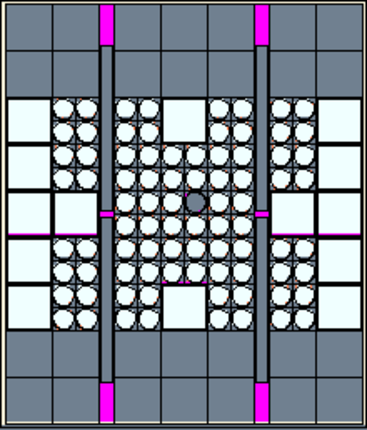
\includegraphics[height=2.2in]{jcore.pdf}
        \caption{}
    \end{subfigure}%
    ~ 
    \begin{subfigure}[t]{0.5\textwidth}
        \centering
        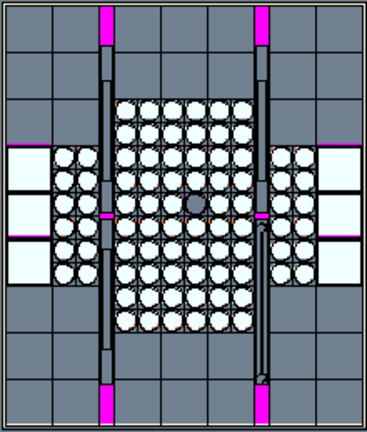
\includegraphics[height=2.2in]{kcore.pdf}
        \caption{}
    \end{subfigure}
    \caption{J core (a) and K core (b) configurations.}
    \label{fig:core_configurations}
\end{figure*}
\subsection{Approach to critical}
Following initial fuel loading in 2009, a criticality experiment was performed and logged. This experiment was performed at low power (cold, clean core). This experiment provided several critical bank heights to test the model against the actual core in various configurations. Starting with a single fuel bundle, reactor lab staff added bundle
s until the core achieved criticality at (18 bundles). After achieving criticality, the staff continued adding fuel until all bundles were in the core. Following the addition of the last bundle, a single reflector was added. The worth of the reflector was tested in various positions in the core grid. Finally, the last reflectors were added over 4 steps.  Figure \ref{fig:atc} shows the model's eigenvalue predictions for the experiment.

\begin{figure}[t!]
  \centering
  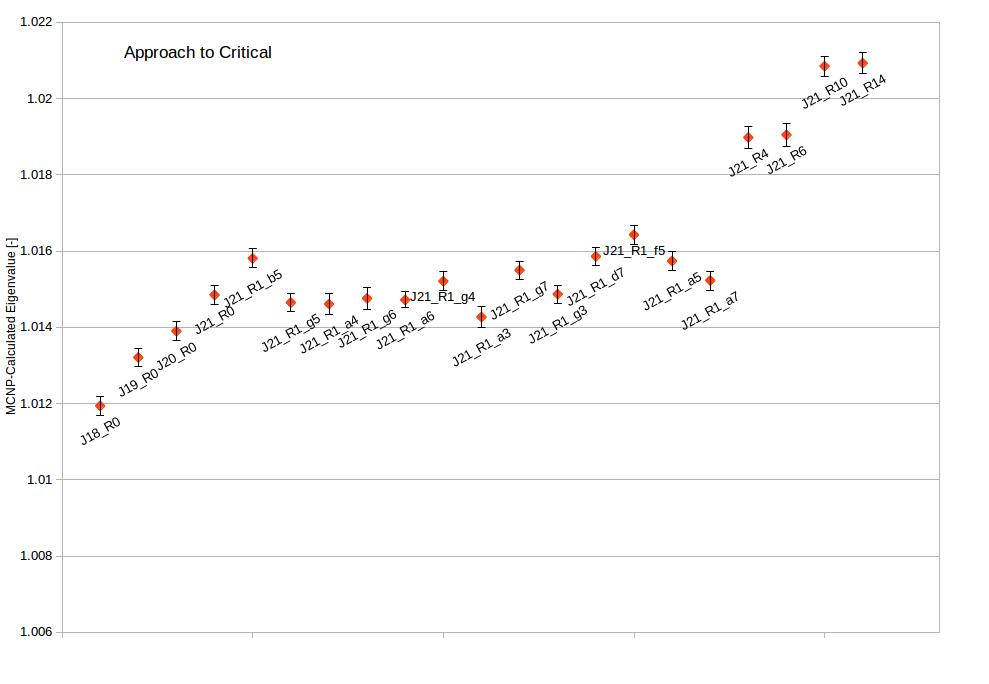
\includegraphics[width=6in]{atc_run_1229.jpg}
  \caption{MCNP eigenvalue calculations at various critical bank heights.}
  \label{fig:atc}
\end{figure}

\noindent
The eigenvalue bias increased with the addition of fuel and reflector elements. The final keff estimate for the full J core configuration (21 bundles, 14 reflectors) was 1.02093 (+/- 0.00027).


\subsection{Initial burnup calculations}
The following figure (\ref{fig:burnup_reactivity}) is the result of preliminary burnup calculations obtained from MCNP6 with various burnup step size (10 days - 100 days) each step with power of 1MW. Burnup analysis was performed for the K core configuration. Isotopes up to Tier 2 were tracked here. KCODE for the calculations was $10^{5}$ histories per cycle, 60 total cycles with 10 cycles discarded. It represents the cold excess reactivity for a fresh core. Further calculations and analysis are to come as enhanced material composition information is applied to the model.
\begin{figure}[H]
  \centering
  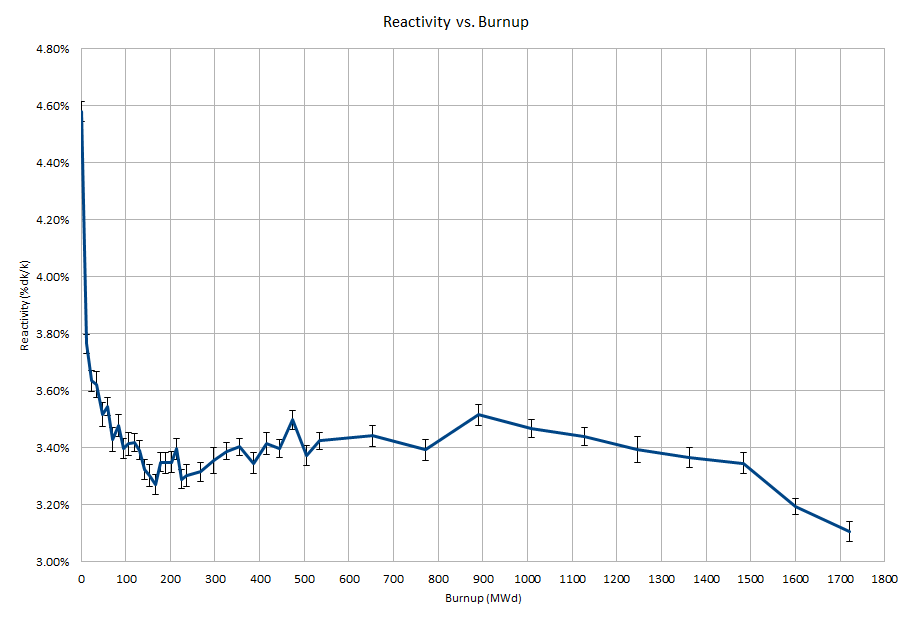
\includegraphics[width=6in]{burnup_fig.png}
  \caption{Reactivity vs. Burnup.}
  \label{fig:burnup_reactivity}
\end{figure}


\subsection{Fuel Composition}
\subsubsection{Fissile material content}
The UWNR Safety Analysis Report (SAR) estimates the average $U^{235}$ content per \emph{pin} element is 149 grams\cite{SAR}. However, the as-built fuel data provided by CERCA shows significant variation in fissile content across the entire core. In reality, there is ~2.2\% deviation in $U^{235}$ content in all the slugs. Figure \ref{fig:235_dist} shows the distribution of fissile material in the core.

\begin{figure}[H]
  \centering
  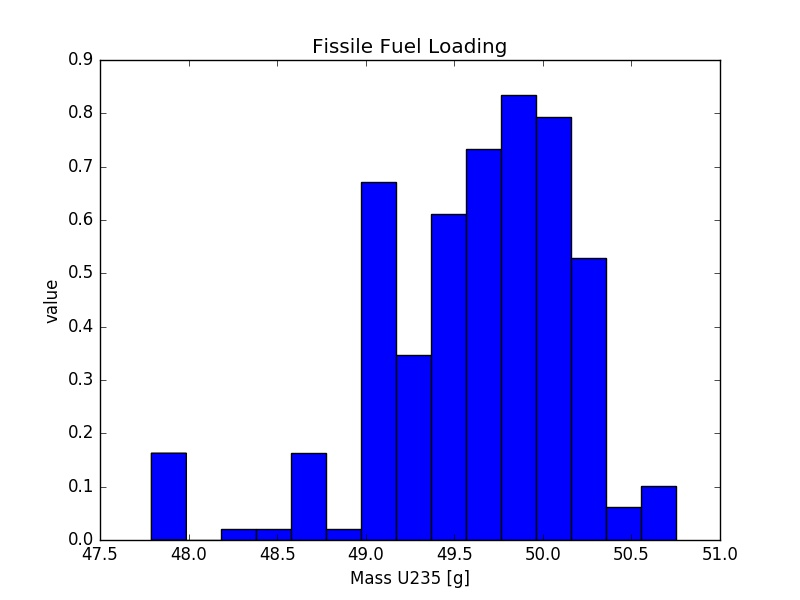
\includegraphics[width=3in]{mass235.jpeg}
  \caption{Fissile material distribution in the fuel slugs.}
  \label{fig:235_dist}
\end{figure}

\noindent
This significant distribution of fissile material in the core led us to believe that a uniform fuel composition scheme was inadequate to model this system.



\subsubsection{Erbium poison content}

TRIGA reactors use Erbium as a burnable poison in their fuel, both to offset excess reactivity and to allow for unique transient behavior\cite{NRAD}. The strong Doppler feedback effects from Erbium allow TRIGA reactors to perform high-power transients (pulses). Erbium also contributes to the overall neutron economy during steady-state operation. Accurate modeling of Erbium absorption in the fuel is crucial to created a successful reactor physics model.

The old MCNP model used average fuel composition values across all fuel slugs, including the average Erbium concentration value from the SAR. The Erbium concentration was set at 0.9\%. Natural abundance was assumed and the appropriate isotopic distributions were applied in the model. This average value was a poor approximation to the actual distribution of Er in the core. Fuel manifests provided by CERCA revealed a large standard deviation in Erbium loading across the core (+/- 7\%). A sensitivity study was performed to gauge the reactivity penalty from a uniform assumption. 

The study compared the inner and outer core regions to compare their reactivity worth. Interestingly, the 9 inner bundles of the core had nearly double the standard deviation as the 12 outer bundles. Fuel definition errors should be more significant in regions of higher flux, this was the motivation for the comparison. Table \ref{tab:erbium_results} contains the results of the regional comparisons.
\begin{table}[h]
  \centering
  \caption{Erbium Sensitivity: Reactivity worth of the standard deviation}
  \begin{tabular}{lcccc}
    \toprule
    Inner Core & 90\% & 100\% & 110\% & Worth \tablefootnote{Worth is normalized to number of pins in region.}$[\frac{\Delta k}{k}]$ \\
    \midrule
    Eigenvalue & \num{0.95375} & \num{0.94748} & \num{0.94051} & \num{-0.014} \\
    St. Dev. & \num{0.00044} & \num{0.00052} & \num{0.0005} & \num{} \\
    \midrule
    \midrule
    Outer Core &  &  &  &   \\
    \midrule
    Eigenvalue & \num{0.95137} & \num{0.94748} & \num{0.94333} & \num{-0.0085} \\
    St. Dev. & \num{0.00058} & \num{0.00052} & \num{0.00049} & \num{} \\ 
    \bottomrule
  \end{tabular}
  \label{tab:erbium_results}
\end{table}

This analysis slightly over-estimated the significance of the uniform Er mass approximation. The analysis was performed for a +/- 10\% mass deviation, in reality, the interval is +/- 7.5\%. Regardless, Er concentrations vary too much (especially the inner 9 bundles) to be approximated as uniform.

 

\subsubsection{Hydride content}

TRIGA fuel is unique in that, much of the moderation in a TRIGA reactor occurs in the fuel itself. Following fabrication, the fuel is hydrided, adding moderating power to the fuel meat. Hydride concentration has a large impact on the thermal flux distribution in the fuel. Again, the SAR estimates this hydride mass as uniform across the core. In reality, the hydride composition varies. The hydride concentration was varied by +/-10\% to determine the effects of this variation. The effect was less pronounced than the Er deviation, the worth over the 10\% range was 0.0032 $[\frac{\Delta k}{k}]$.

\subsubsection{Fuel composition conclusion}

There is significant variation in fuel composition across all fuel slugs in UWNR. The non-uniformity of the fuel leads to significant reactivity bias when running the model with core-averaged values. The model now accounts for the as-built fuel data. The scripts used to build the input files parse the fuel data so each pin has its own unique, accurate (to manufacturer specifications) material definition in MCNP. The above composition issues have been accounted for.
 







%%%%%%%%%%%%%%%%%%%%%%%%%%%%%%%%%%%%%%%%%%%%%%%%%%%%%%%%%%%%%%%%%%%%%
\section{Future Work}

\subsection{Temperature Mapping}

UWNR has temperature maps available for the operating core. It will be important for burnup analysis to implement the radial and axial fuel temperature profiles, as well as the coolant temperature profile. These profiles will be used as an input to select the proper MCNP cross-section libraries, and to define correct material densities. 

\subsection{PyNE Implementation}

Eventually, the code will fully implement the nuclear engineering toolkit for material definitions. This will ensure uniform material definitions.


%%%%%%%%%%%%%%%%%%%%%%%%%%%%%%%%%%%%%%%%%%%%%%%%%%%%%%%%%%%%%%%%%%%%%




%%%%%%%%%%%%%%%%%%%%%%%%%%%%%%%%%%%%%%%%%%%%%%%%%%%%%%%%%%%%%%%%%%%%%
\setlength{\baselineskip}{12pt}

\bibliographystyle{UWNR_modeling}
\bibliography{references}

%%%%%%%%%%%%%%%%%%%%%%%%%%%%%%%%%%%%%%%%%%%%%%%%%%%%%%%%%%%%%%%%%%%%%
\newpage
\appendix
\begin{figure}[H]
  \centering
  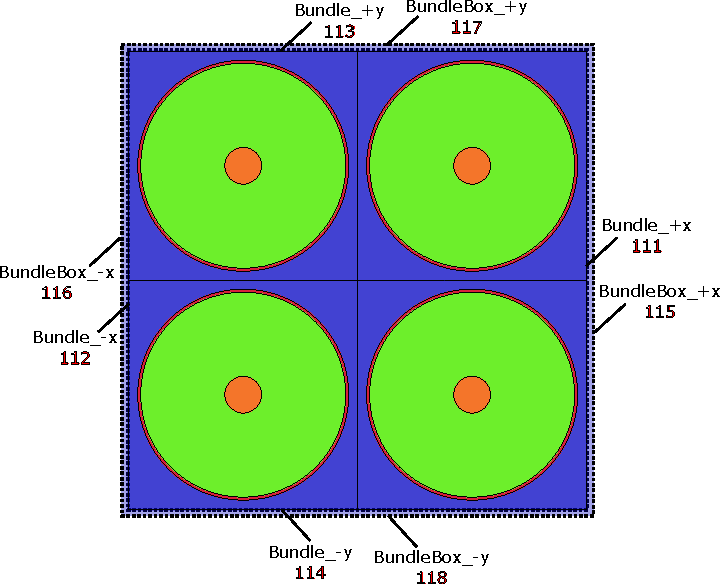
\includegraphics[width=5in]{bundle_xy.pdf}
  \caption{Fuel bundles, horizontal view.}
  \label{fig:bundle_xy}
\end{figure}
\begin{figure}[H]
  \centering
  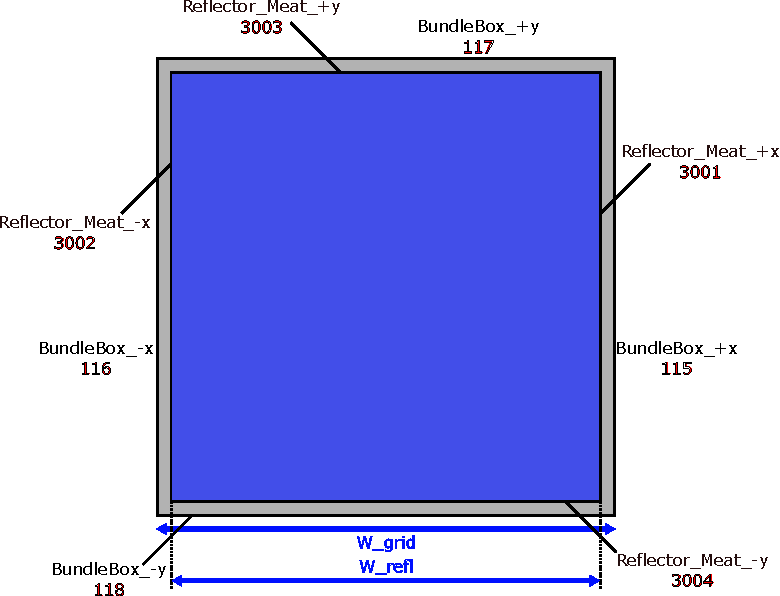
\includegraphics[width=5in]{Refl_xy.pdf}
  \caption{Reflector element, horizontal view.}
  \label{fig:Refl_xy}
\end{figure}
\begin{figure}[H]
  \centering
  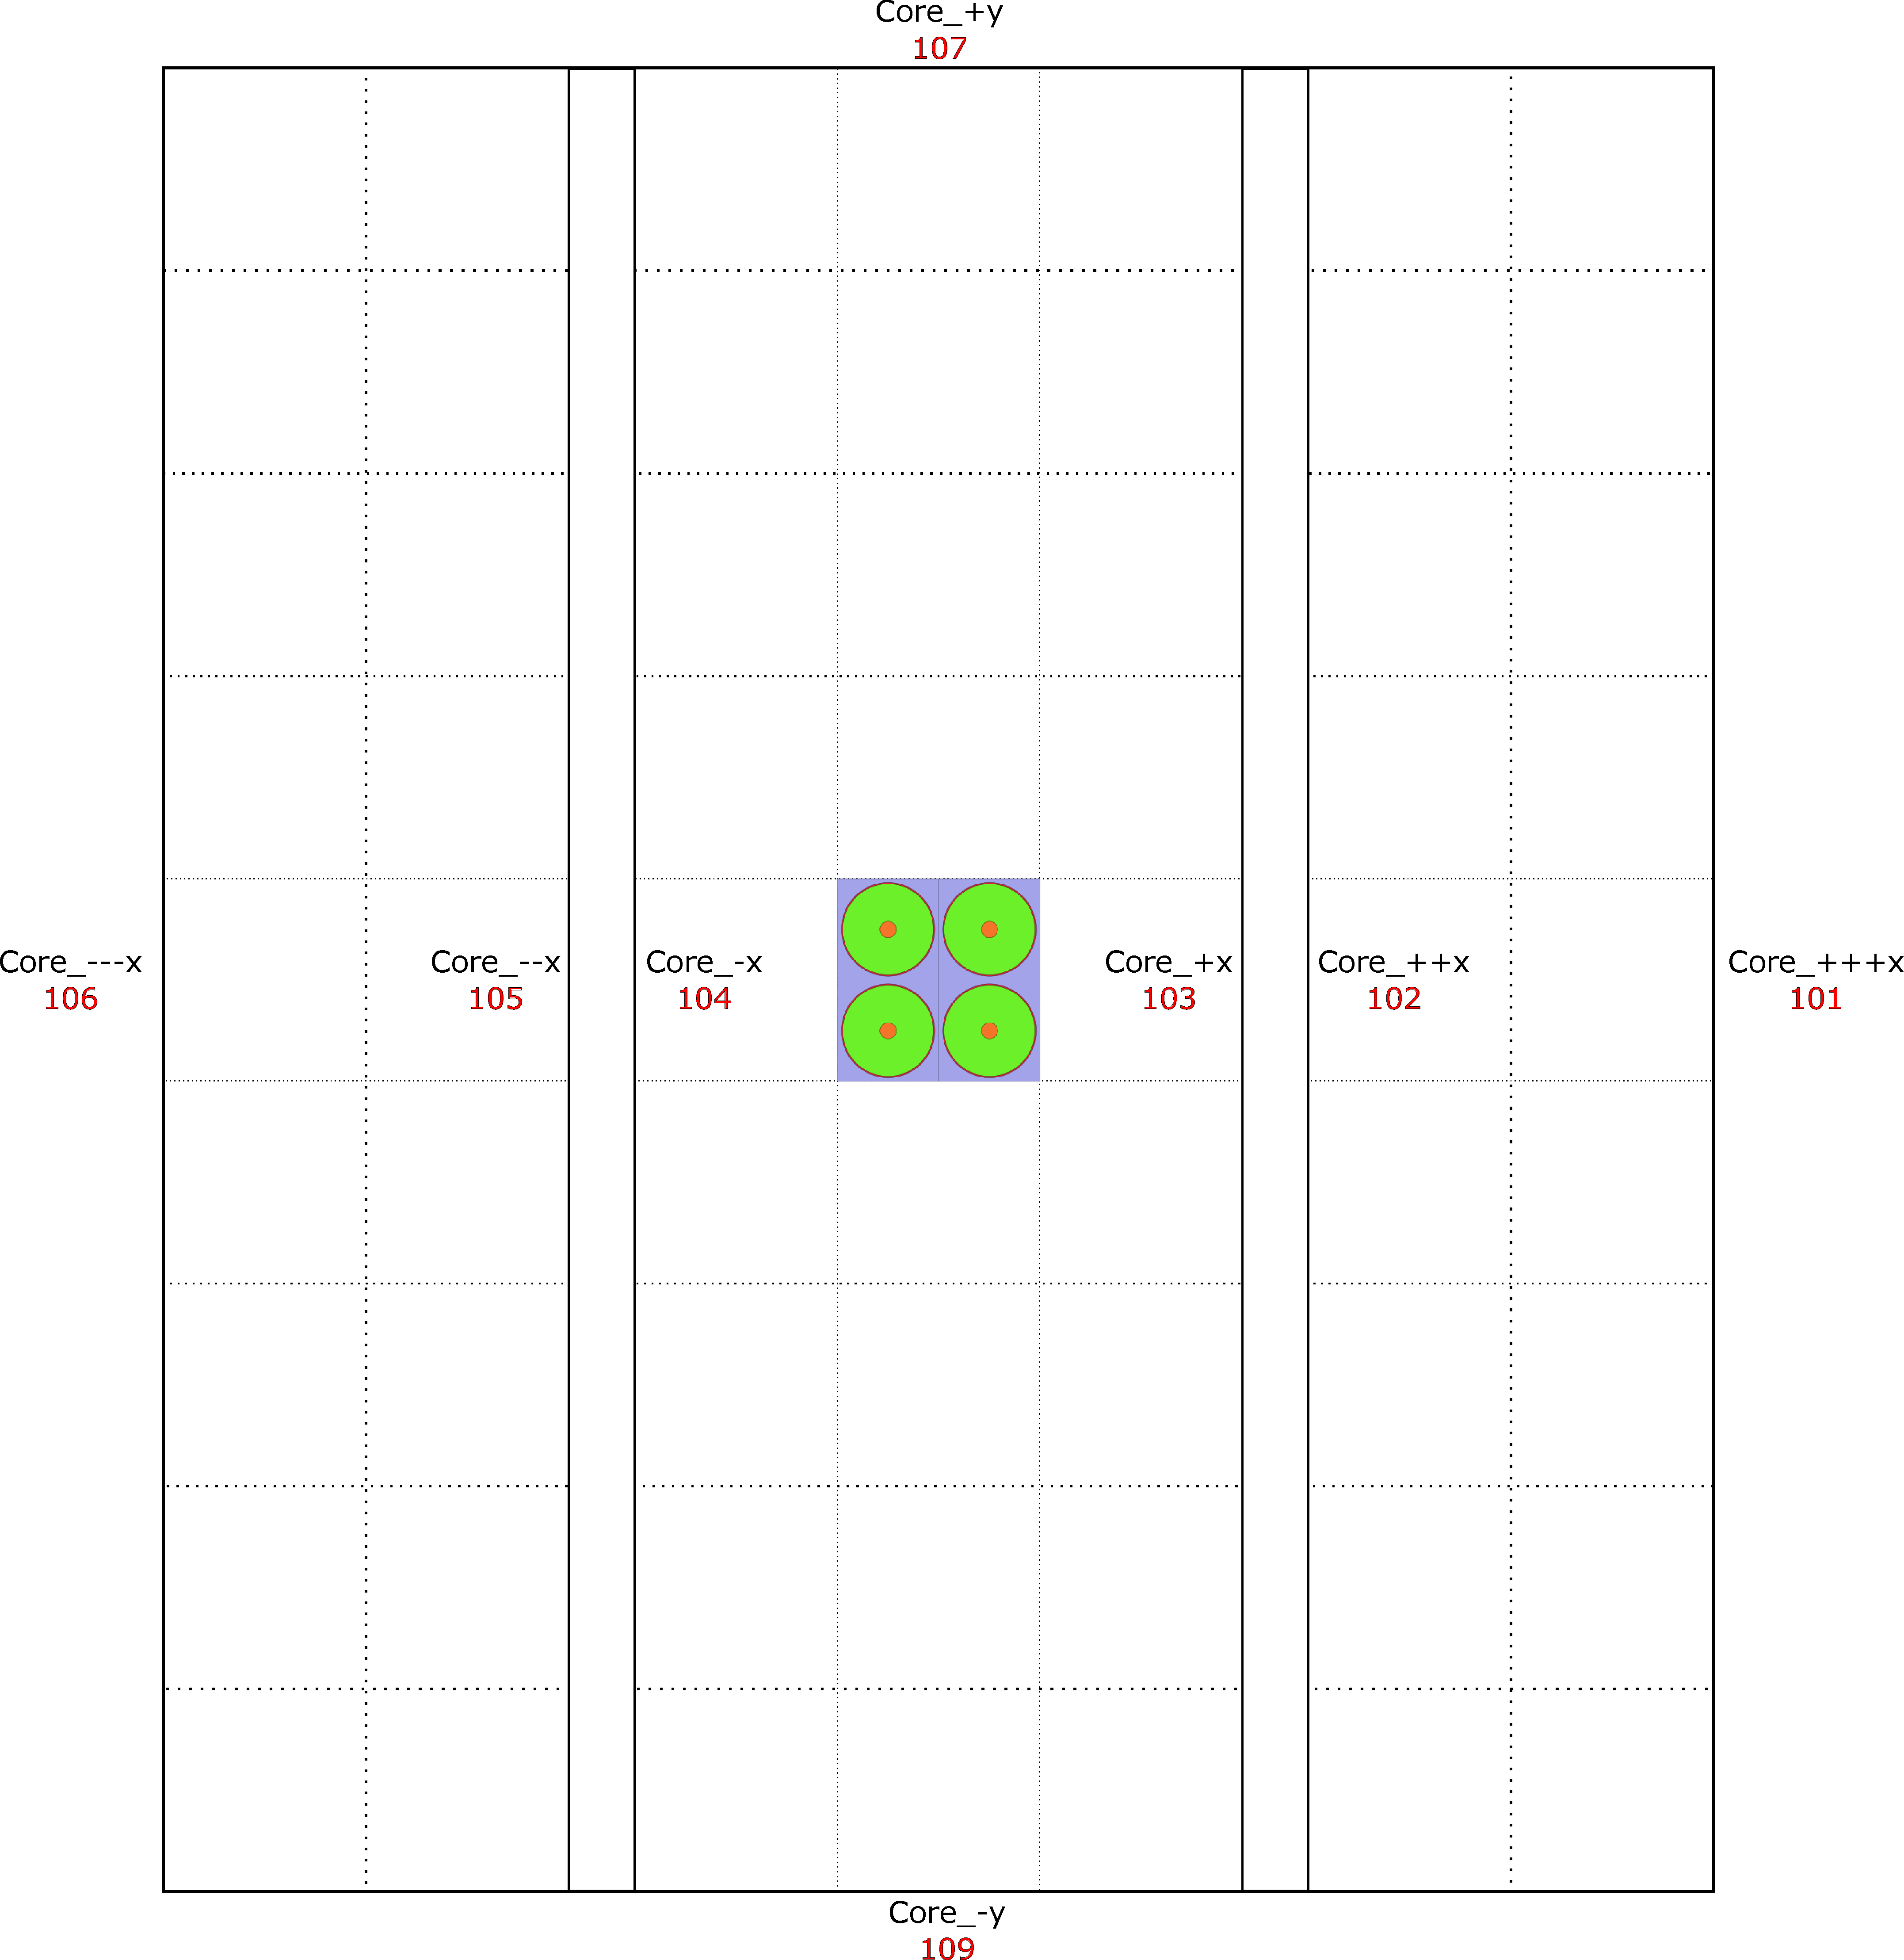
\includegraphics[width=7in]{core_xy.pdf}
  \caption{Core regions, horizontal view.}
  \label{fig:core_xy}
\end{figure}
\begin{figure}[H]
  \centering
  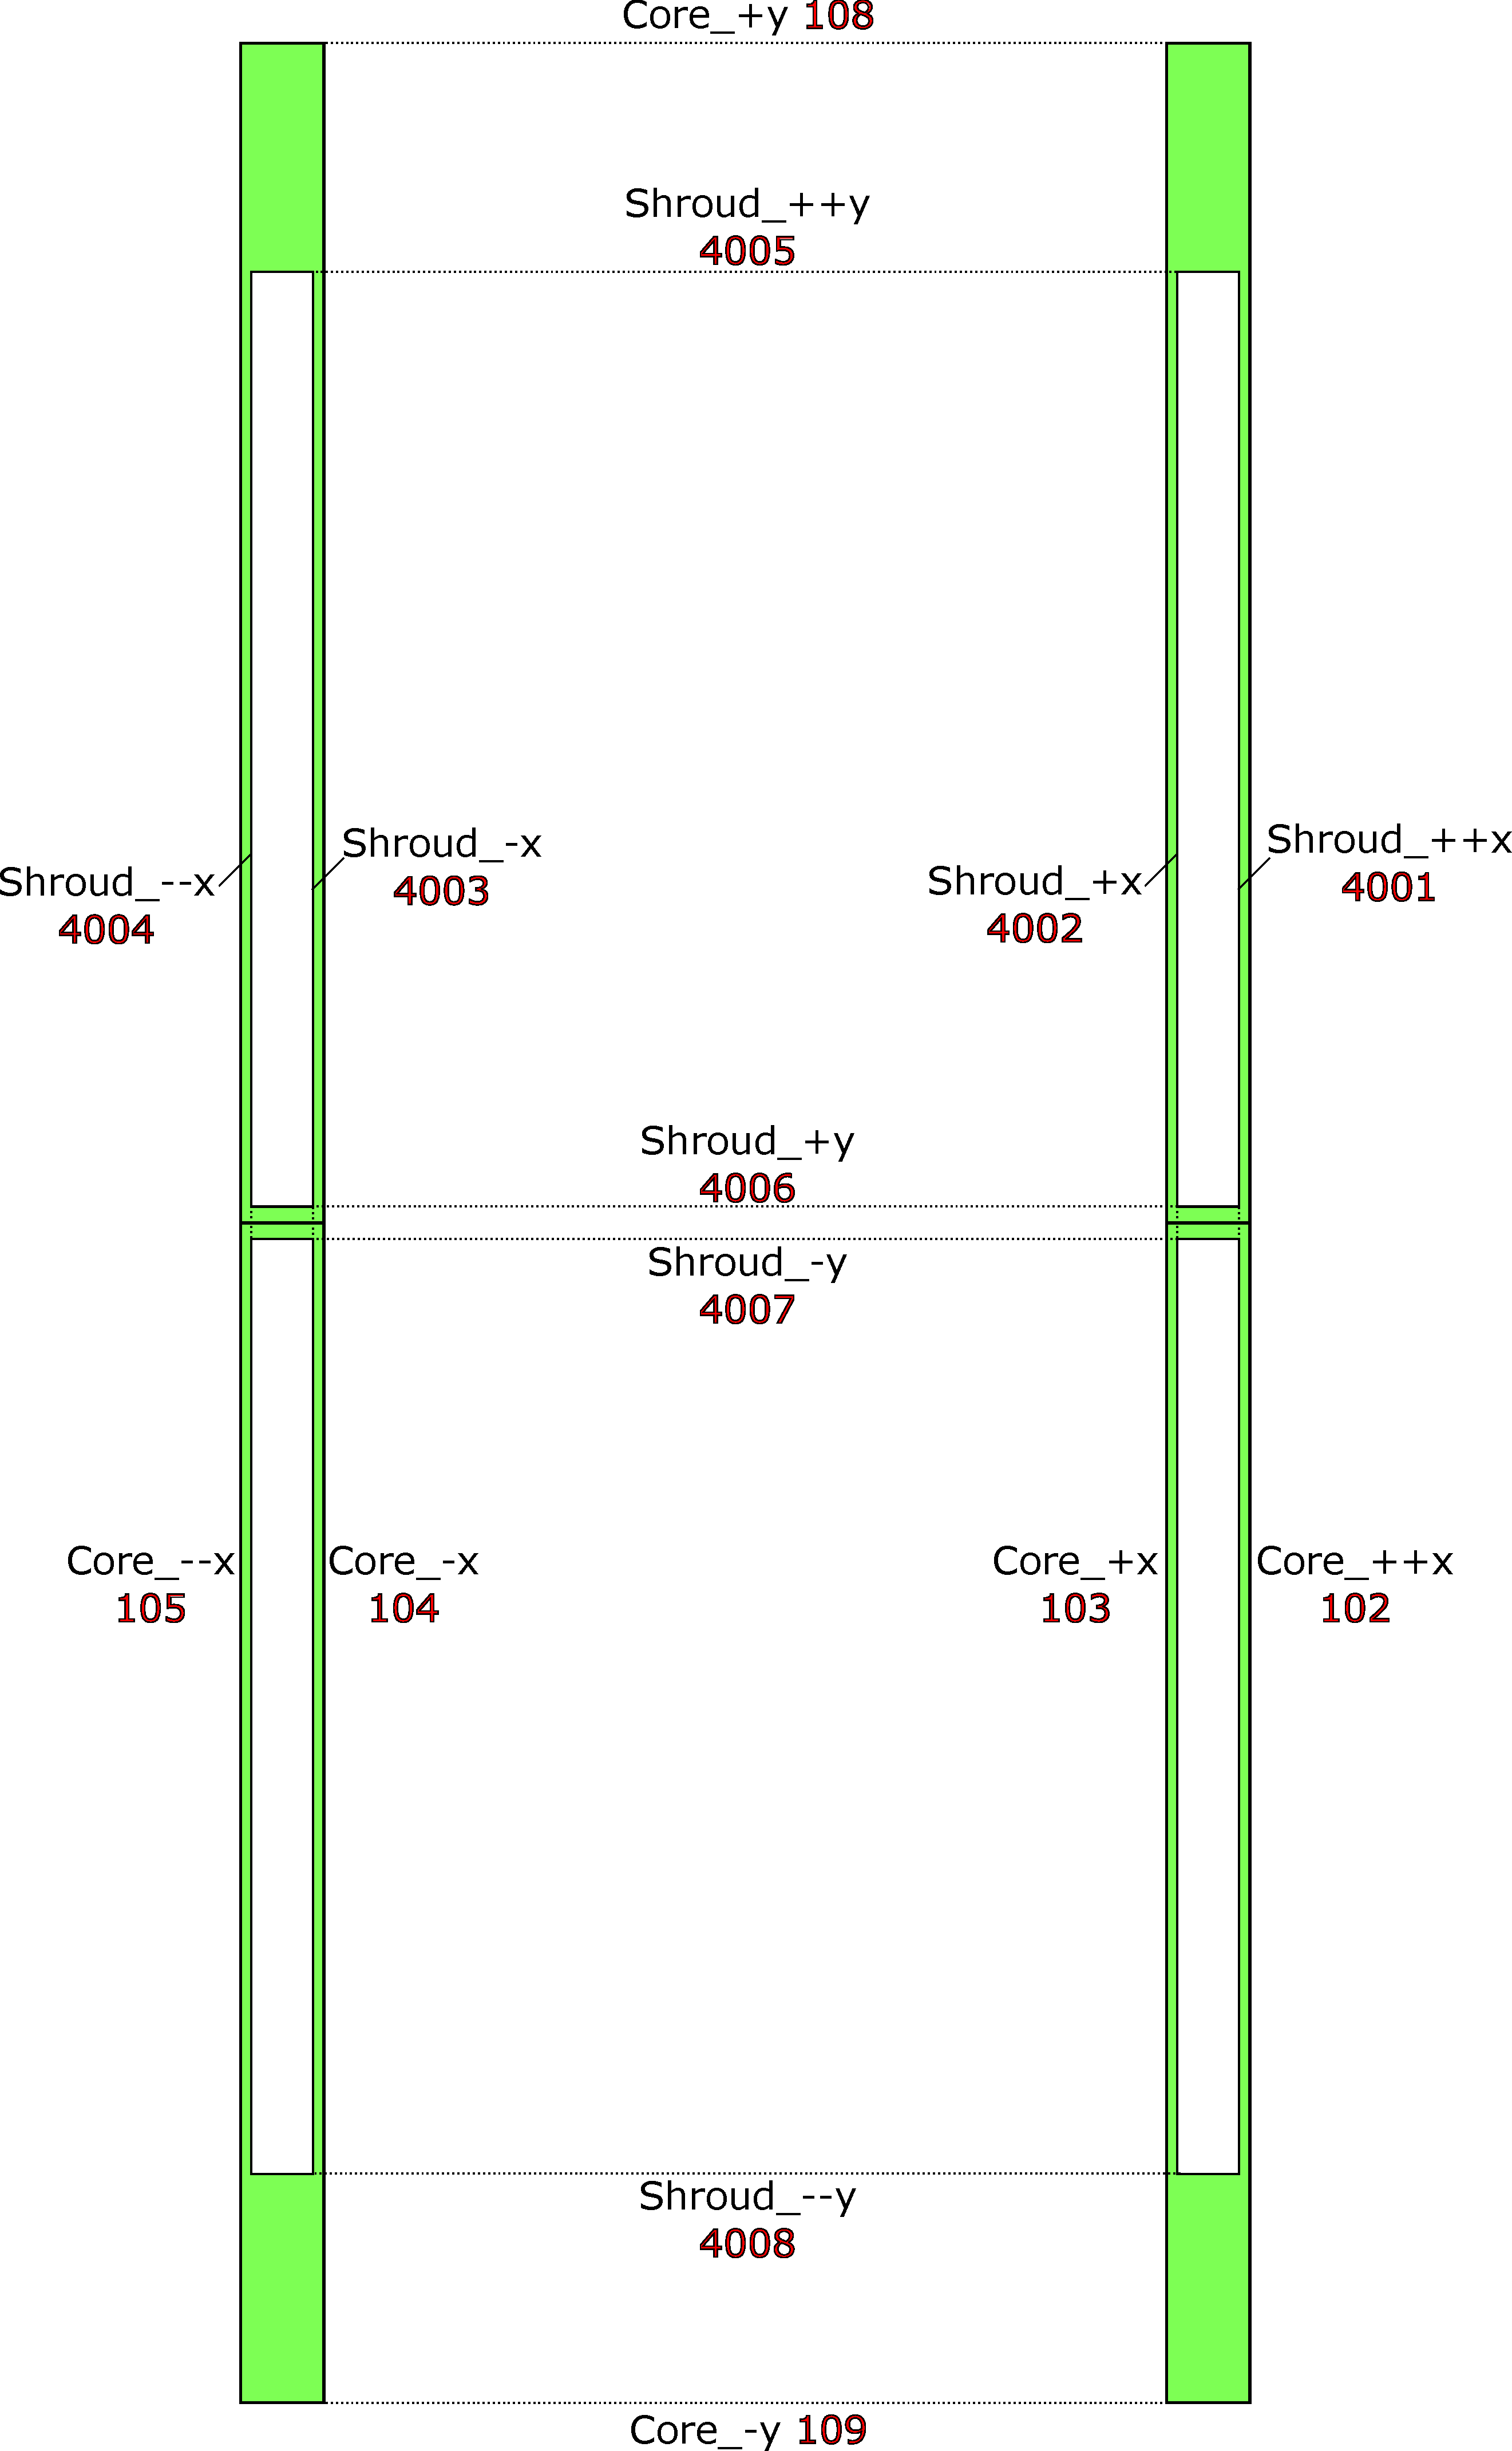
\includegraphics[width=5.5in]{CS_xy.pdf}
  \caption{Control shroud, horizontal view.}
  \label{fig:CS_xy}
\end{figure}
\begin{figure}[H]
  \centering
  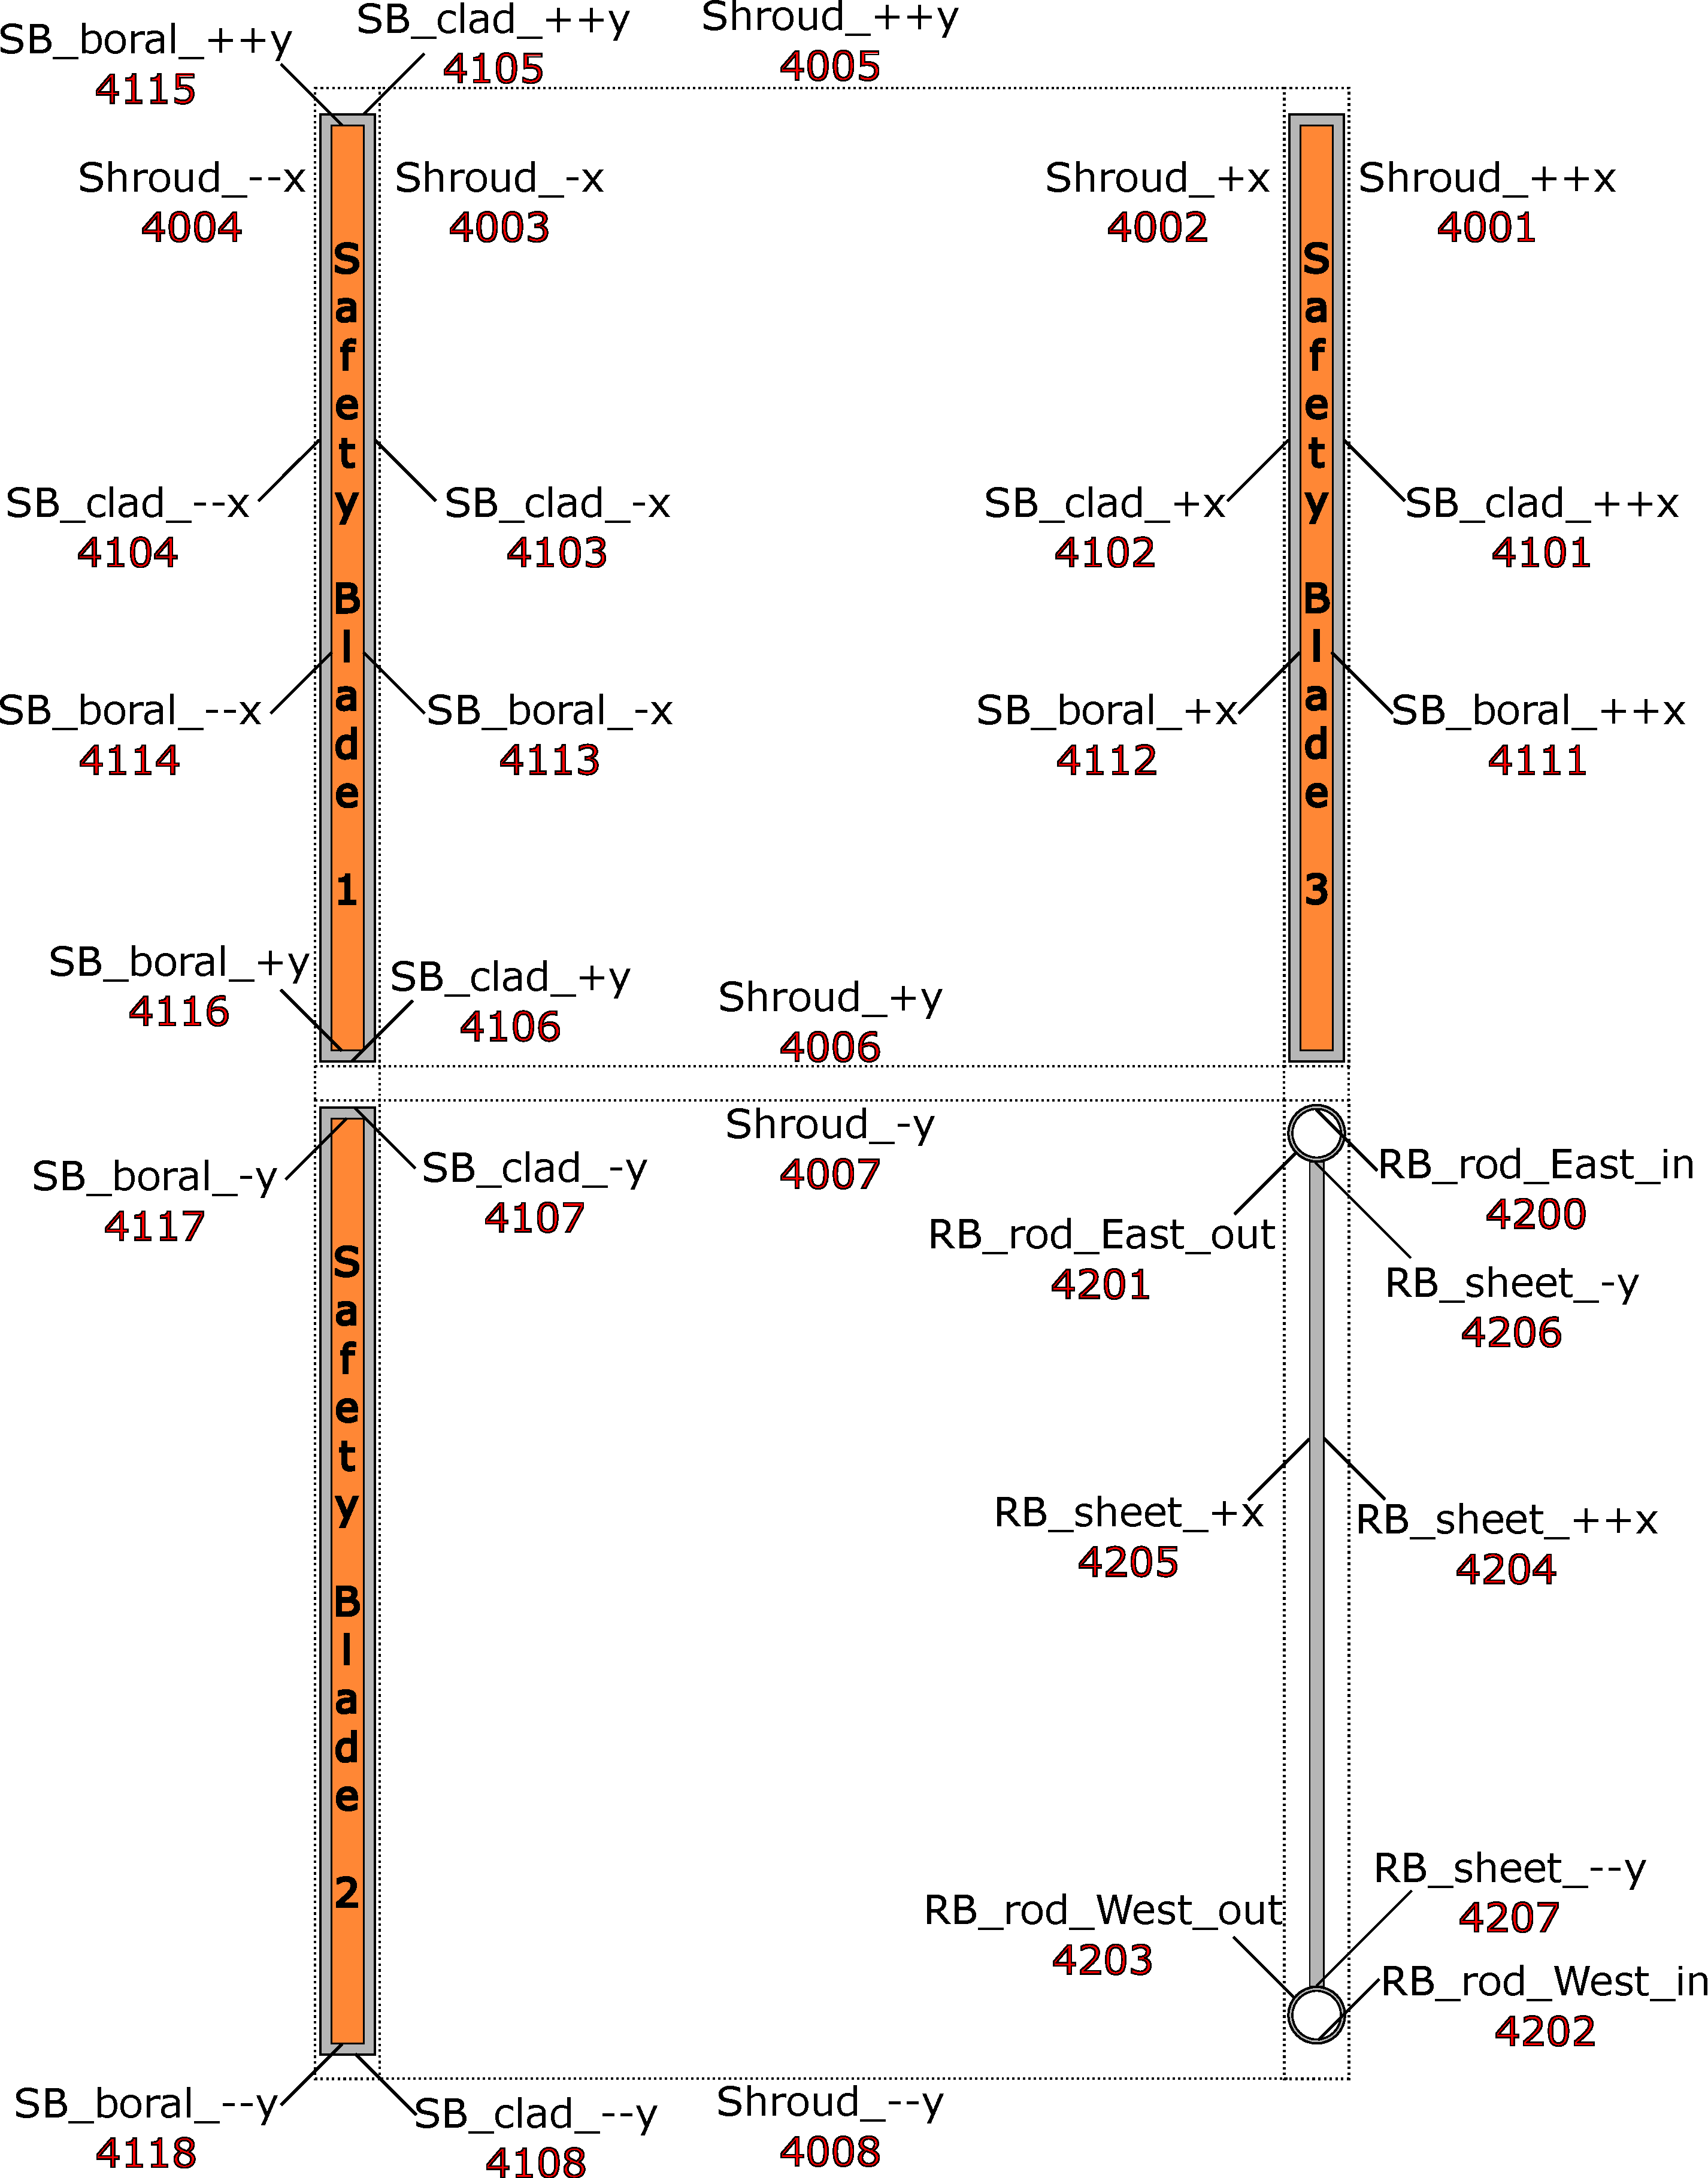
\includegraphics[width=7in]{SBRB_xy.pdf}
  \caption{Safety Blades and Regulating blade, horizontal view.}
  \label{fig:SBRB_xy}
\end{figure}
\begin{figure}[H]
  \centering
  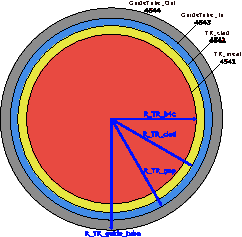
\includegraphics[width=3in]{TR_xy.pdf}
  \caption{Transient rod, horizontal view.}
  \label{fig:TR_xy}
\end{figure}
\end{document}
